\documentclass[12pt,UTF8,fleqn]{ctexart}
\usepackage{ctex,amsmath,amssymb,geometry,fancyhdr,bm,amsfonts,mathtools,extarrows,graphicx,url,enumerate,xcolor,float,multicol,wasysym}
\usepackage{subfigure}
\allowdisplaybreaks[4]
% 加入中文支持
\newcommand\Set[2]{\left\{#1\ \middle\vert\ #2 \right\}}
\newcommand\Lim[0]{\lim\limits_{n\rightarrow\infty}}
\newcommand\LIM[2]{\lim\limits_{#1\rightarrow#2}}
\newcommand\Ser[1]{\sum_{n=#1}^\infty}
\newcommand{\SER}[2]{\sum_{#1=#2}^\infty}
\newcommand{\Int}[4]{\varint\nolimits_{#1}^{#2}#3\mathrm d#4}
\newcommand{\aIInt}[1]{\iint\limits_{#1}}
\newcommand{\IInt}[3]{\iint\limits_{#1}#2\mathrm d#3}
\newcommand{\varIInt}[4]{\iint\limits_{#1}#2\mathrm d#3\mathrm d#4}
\newcommand{\IIInt}[3]{\iiint\limits_{#1}#2\mathrm d#3}
\newcommand{\varIIInt}[5]{\iiint\limits_{#1}#2\mathrm d#3\mathrm d#4\mathrm d#5}
\newcommand{\LInt}[3]{\varint\nolimits_{#1}#2\mathrm d#3}
\newcommand{\LOInt}[3]{\varoint\nolimits_{#1}#2\mathrm d#3}
\newcommand{\LLInt}[4]{\varint\nolimits_{#1}\nolimits^{#2}#3\mathrm d#4}
\newcommand{\BLInt}[2]{\varint\nolimits_{#1}#2}
\newcommand{\varBLInt}[3]{\varint\nolimits_{#1}\nolimits^{#2}#3}
\newcommand{\BLOInt}[2]{\varoint\nolimits_{#1}#2}
\newcommand{\SIInt}[3]{\iint\limits_{#1}#2\mathrm d#3}
\newcommand{\md}[1]{\mathrm d#1}
\newcommand{\BSIInt}[2]{\iint\limits_{#1}#2}
\newcommand{\pp}[2]{\frac{\partial #1}{\partial #2}}
\newcommand{\ppx}[1]{\frac{\partial #1}{\partial x}}
\newcommand{\ppy}[1]{\frac{\partial #1}{\partial y}}
\newcommand{\ppz}[1]{\frac{\partial #1}{\partial z}}
\newcommand{\varppx}[1]{\frac{\partial}{\partial x} #1}
\newcommand{\varppy}[1]{\frac{\partial}{\partial y} #1}
\newcommand{\varppz}[1]{\frac{\partial}{\partial z} #1}
\newcommand{\BSOIInt}[2]{\oiint\limits_{#1}#2}
\newcommand{\me}[0]{\mathrm e}
\geometry{a4paper,scale=0.80}
\pagestyle{fancy}
\rhead{常微分方程(2)}
\lhead{基础习题课期末复习}
\chead{微积分B(2)}
\begin{document}
\setcounter{section}{16}
\section{高阶线性微分方程解的结构}
\subsection{复习计划}
\begin{figure}[H]
\begin{center}
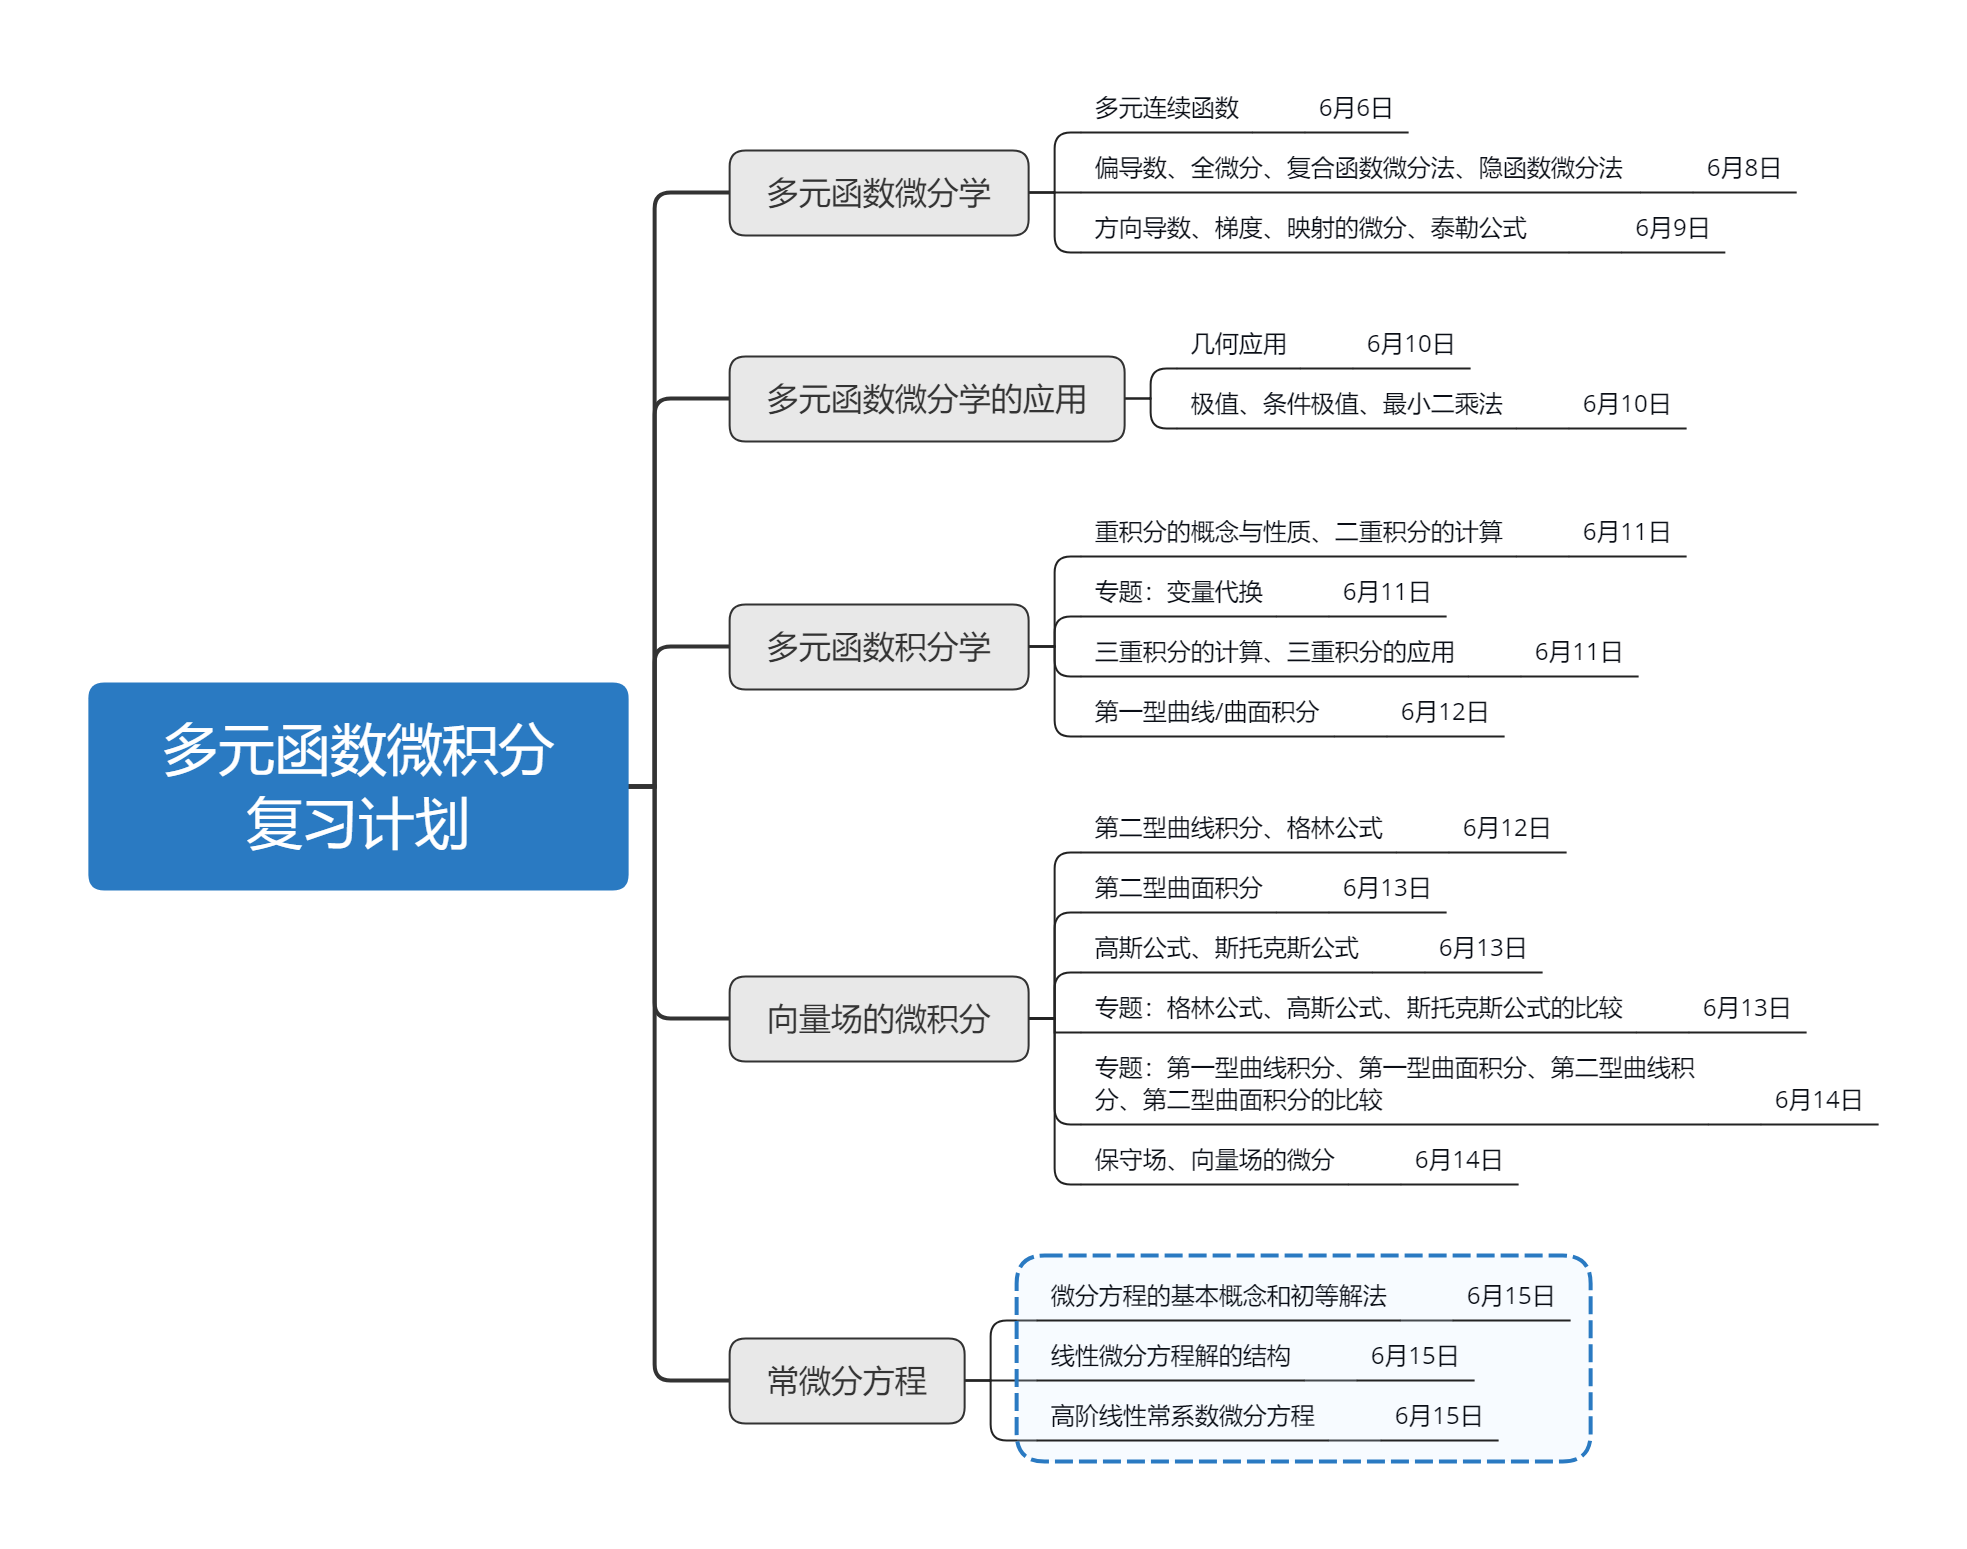
\includegraphics[height=0.5\textheight]{Figures20190615/plan.png}
\end{center}
\end{figure}
\subsection{知识结构}
\begin{figure}[H]
\begin{center}
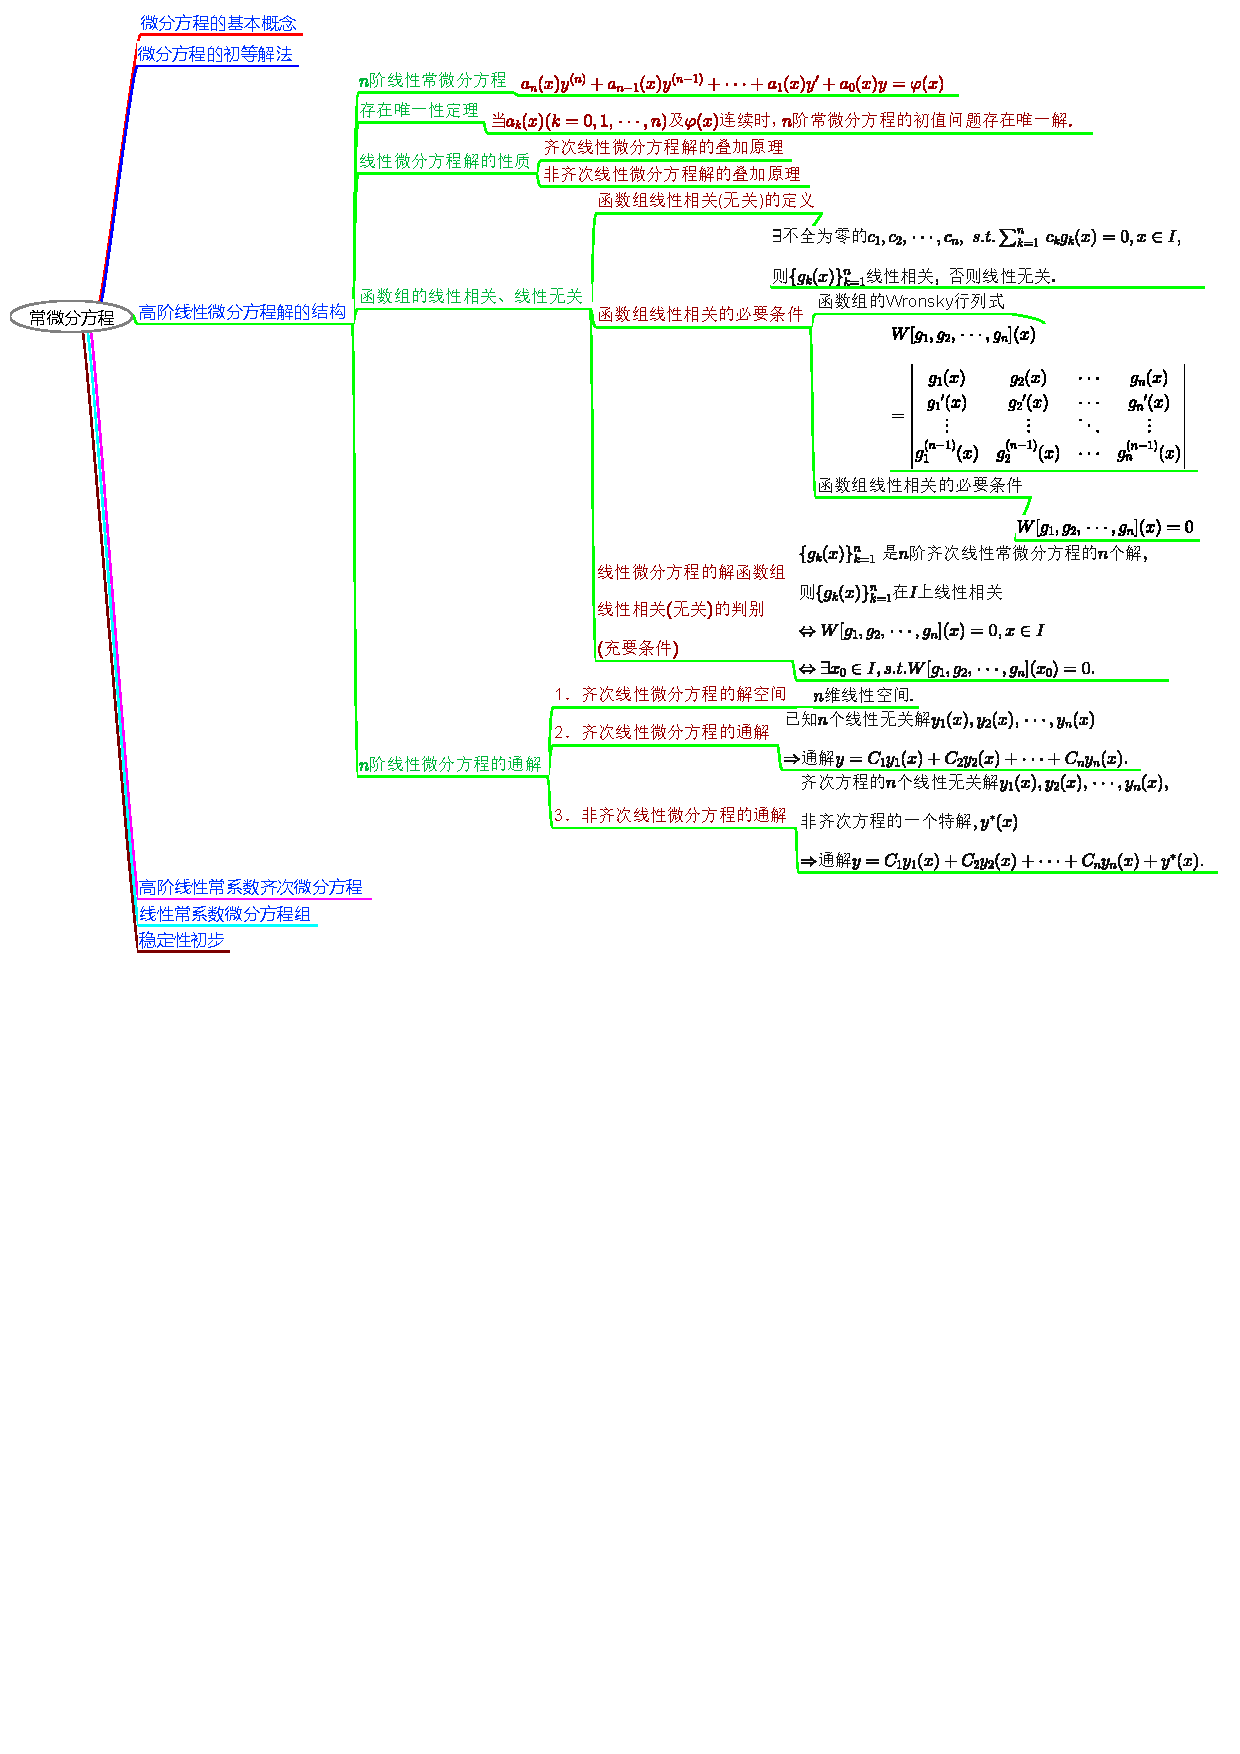
\includegraphics[height=1\textheight]{20190615-1.pdf}
\end{center}
\end{figure}
%\subsection{高阶线性微分方程解的结构}
%\begin{figure}[H]
%\begin{center}
%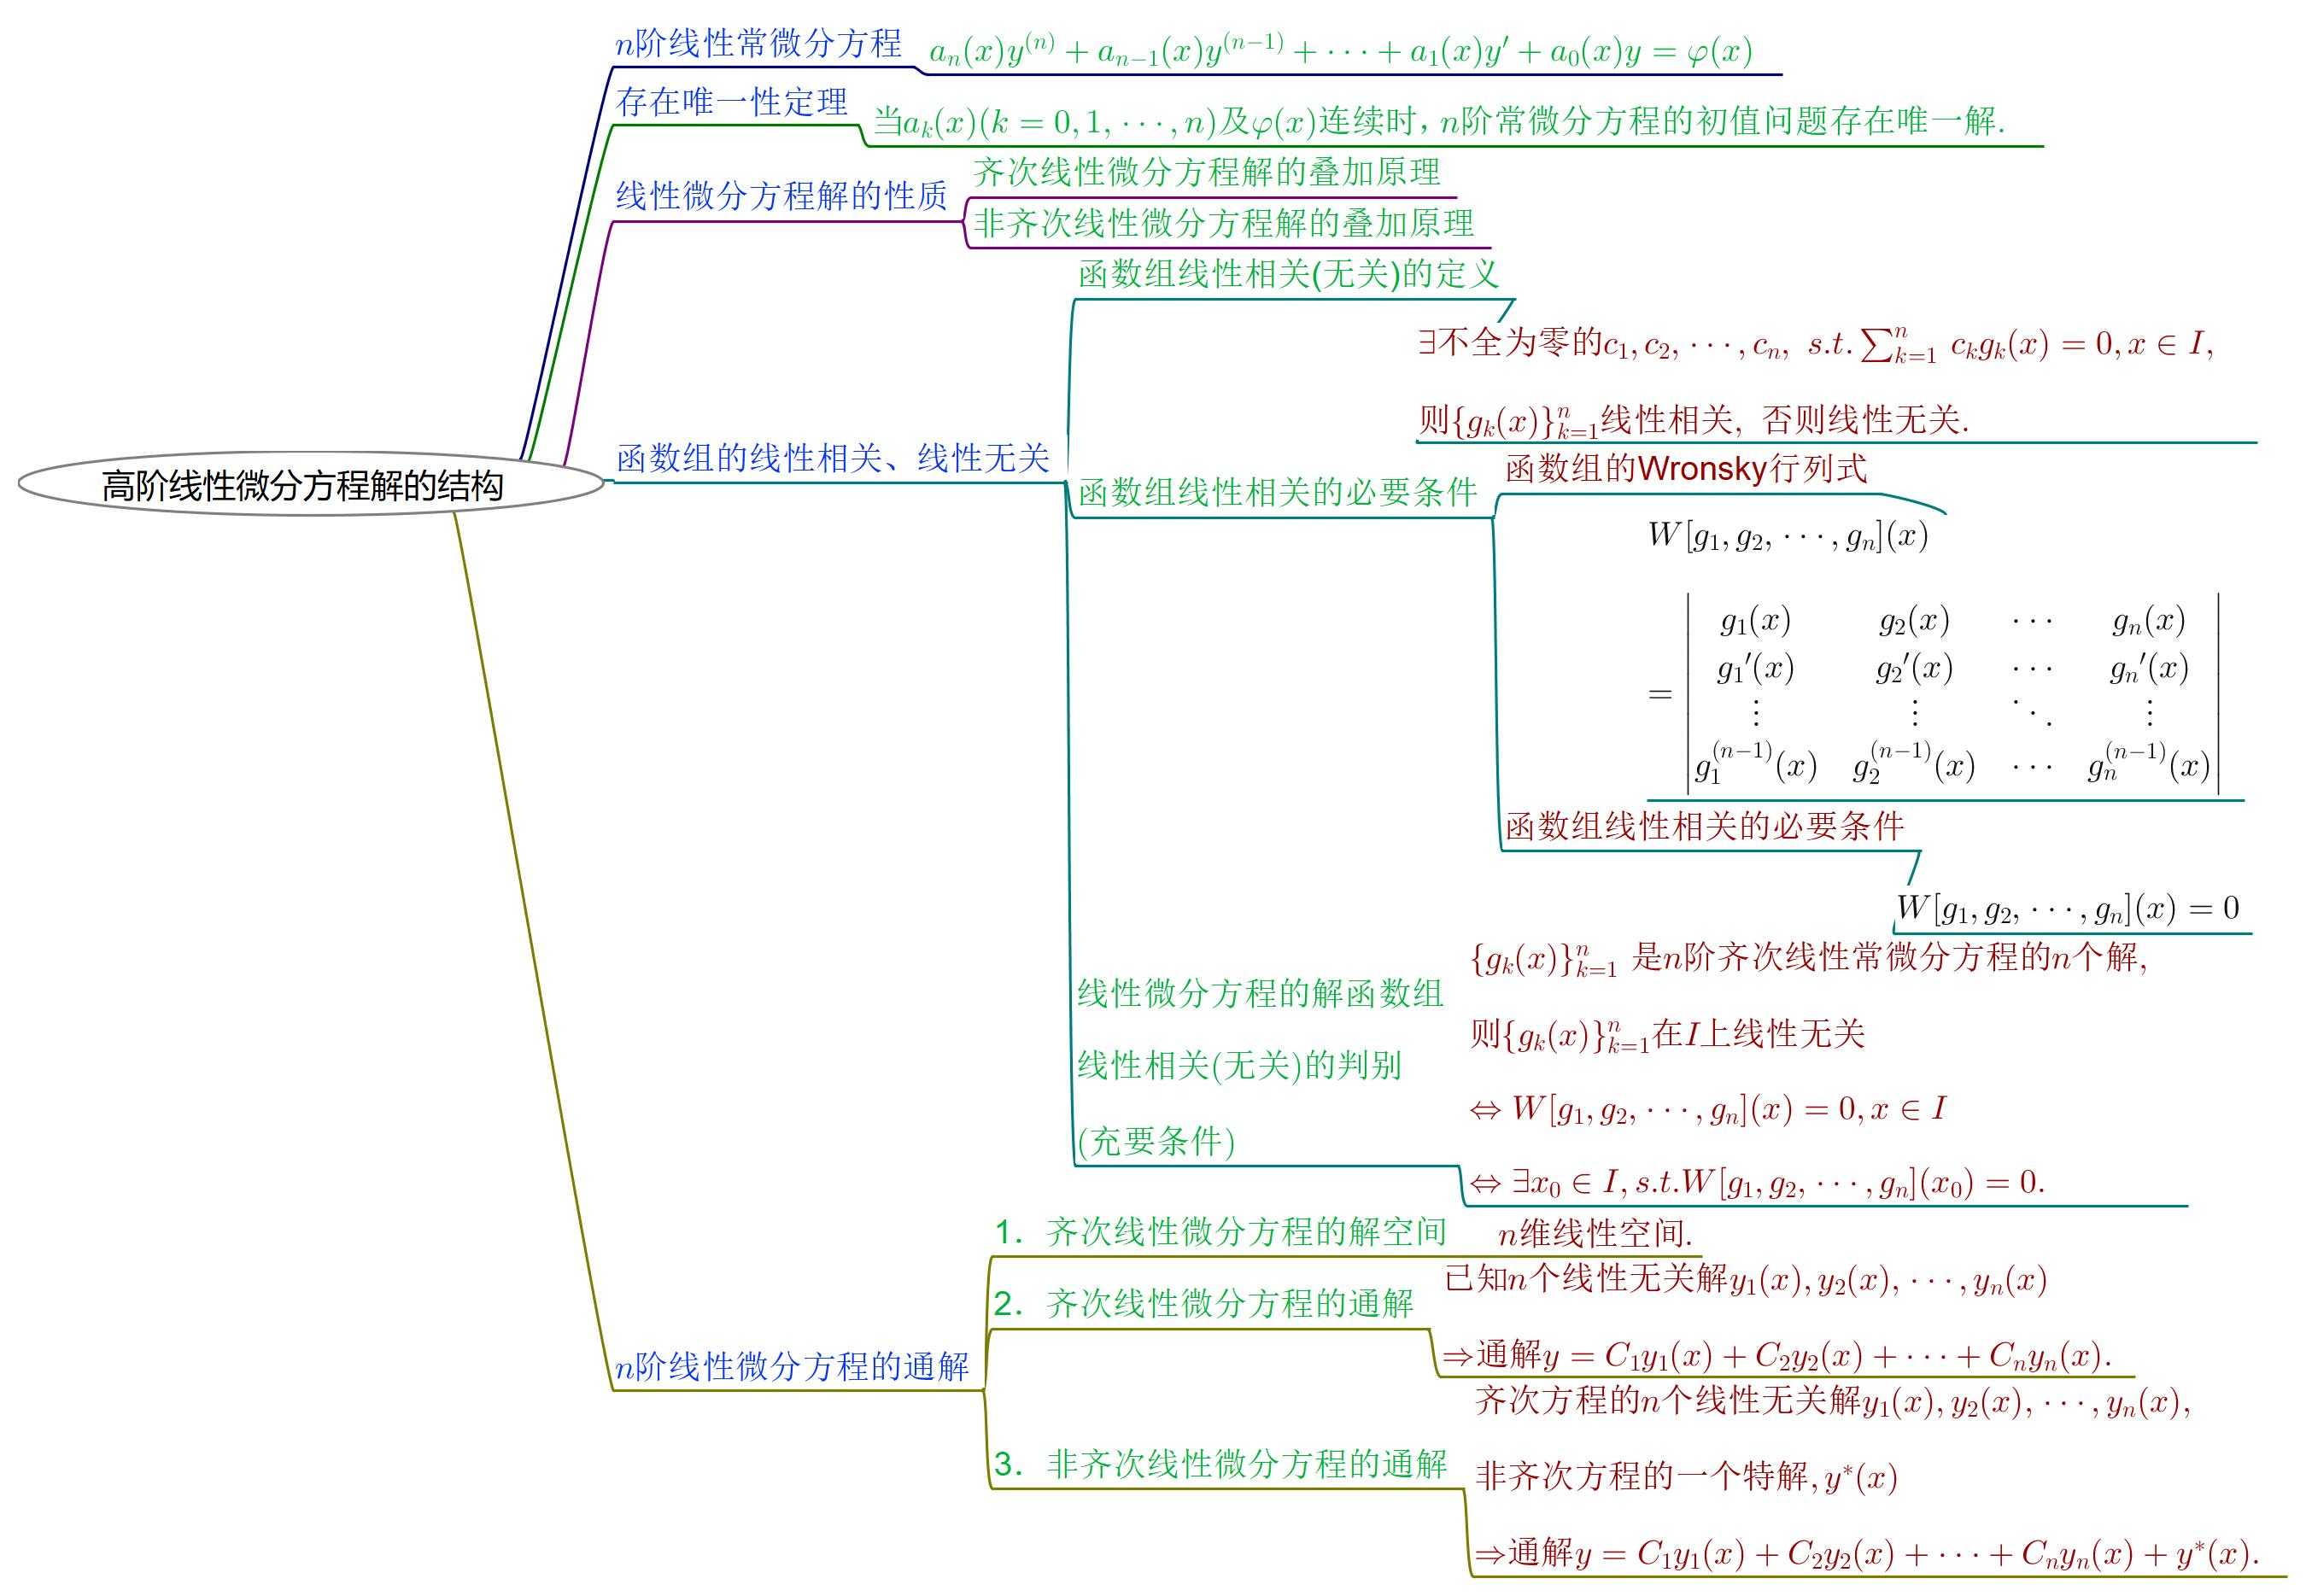
\includegraphics[height=0.5\textheight]{structures-1.jpg}
%\end{center}
%\end{figure}
\subsection{习题分类与解题思路}
\begin{enumerate}
\item判断函数组在定义区间内是否线性相关. 可参考以下思路:
\begin{enumerate}
\item[第一步]计算Wronsky行列式. 若Wronsky行列式不恒等于零,则函数组线性无关.

【如习题14.3中的1.(1)/(2)/(3)/(4)/(5)/(6).】
\item[第二步]若Wronsky行列式恒等于零,则可按照线性相关的定义,判断是否存在不全为零的$c_1,c_2,\cdots,c_n\in\mathbb R$使得$\sum_{i=1}^nc_ng_n(x)=0$,若存在则线性相关,若不存在则线性无关.

若已知函数组是$n$阶线性微分方程的解函数组,则由Wronsky行列式恒等于零,可直接得到该函数组线性相关.
\end{enumerate}
\item考查齐次和非齐次线性方程解的叠加原理. 

【如习题14.3中的3.】
\item考查线性微分方程解的存在唯一性定理.

【如习题14.3中的6.】
\item考查$n$阶线性微分方程的解函数组线性相关(无关)判别的充要条件.

【如习题14.3中的7.】
\item考查$n$阶齐次线性微分方程解的结构. $n$阶齐次线性微分方程的解空间是$n$维线性空间,找到该齐次线性微分方程的$n$个线性无关的解,就可写出该齐次线性微分方程的通解.

【如习题14.3中的2.】
\item考查$n$阶非齐次线性微分方程解的结构. 先确定该非齐次方程对应的齐次方程的$n$个线性无关的解,从而求出齐次方程的通解,加上该非齐次方程的一个特解即可得到该非齐次方程的通解.

【如习题14.3中的8.】
\item其他类型的题目. 利用Wronsky行列式证明$n$阶非齐次线性微分方程有$n+1$个线性无关的解.

【如习题14.3中的9.】
\end{enumerate}
\subsection{习题14.3解答}
\begin{enumerate}
\item判断下列函数组在其定义区间内是否线性相关:\\
\begin{tabular}{ll}
(1)$1,x,x^2,x^3,x^4$;&(2)$\me^{-x},1,\me^x$;\\
(3)$\me^x,x\me^x$;&(4)$\sin x,\cos x$;\\
(5)$\me^x\cos x,\me^x\sin x$;&(6)$\ln x,x\ln x$.
\end{tabular}

解:(1)$W[1,x,x^2,x^3,x^4](x)=\begin{vmatrix}
1&x&x^2&x^3&x^4\\
0&1&2x&3x^2&4x^3\\
0&0&2&6x&12x^2\\
0&0&0&6&24x\\
0&0&0&0&24\\
\end{vmatrix}=1\cdot1\cdot2\cdot6\cdot24\not\equiv0$,

故$1,x,x^2,x^3,x^4$线性无关.

(2)$W[\me^{-x},1,\me^x](x)=\begin{vmatrix}
\me^{-x}&1&\me^x\\
-\me^{-x}&0&\me^x\\
\me^{-x}&0&\me^x
\end{vmatrix}=(-1)^3(-\me^{-x}\me^x-\me^x\me^{-x})=2\not\equiv0$,

故$\me^{-x},1,\me^x$线性无关.

(3)$W[\me^x,x\me^x](x)=\begin{vmatrix}
\me^x&x\me^x\\
\me^x&\me^x(x+1)
\end{vmatrix}=\me^{2x}(x+1)-x\me^{2x}=\me^{2x}\not\equiv0$,

故$\me^x,x\me^x$线性无关.

(4)$W[\sin x,\cos x](x)=\begin{vmatrix}\sin x&\cos x\\\cos x&-\sin x\end{vmatrix}=-1\not\equiv0$,

故$\sin x,\cos x$线性无关.

(5)$W[\me^x\cos x,\me^x\sin x](x)=\begin{vmatrix}
\me^x\cos x&\me^x\sin x\\
\me^x(\cos x-\sin x)&\me^x(\sin x+\cos x)\\
\end{vmatrix}=\me^x(\sin x\cos x+\cos^2x-\sin x\cos x+\sin^2x)=\me^x\not\equiv0$,

故$\me^x\cos x,\me^x\sin x$线性无关.

(6)$W[\ln x,x\ln x](x)=\begin{vmatrix}\ln x&x\ln x\\ \frac1x&\ln x+1\end{vmatrix}=(\ln x+1)\ln x-\ln x=(\ln x)^2\not\equiv0$,

故$\ln x,x\ln x$线性无关.

\item验证$y_1=\me^{x^2}$与$y_2=x\me^{x^2}$都是方程$y''-4xy'+(4x^2-2)y=0$的解,并写出该方程的通解.

解:$y_1=\me^{x^2},y_1'=\me^{x^2}2x,y_1''=2\me^{x^2}+4x^2\me^{x^2}$,

$y_1''-4xy_1'+(4x^2-2)y_1=2\me^{x^2}+4x^2\me^{x^2}-4x\me^{x^2}2x+(4x^2-2)\me^{x^2}=\me^{x^2}(2+4x^2-8x^2+4x^2-2)=0$,

$y_2=x\me^{x^2},y_2'=\me^{x^2}(1+2x^2),y_2''=\me^{x^2}(4x+2x+4x^3)=\me^{x^2}(6x+4x^3)$,

$y_2''-4xy_2'+(4x^2-2)y_2=\me^{x^2}(6x+4x^3)-4x\me^{x^2}(1+2x^2)+(4x^2-2)x\me^{x^2}\\
=\me^{x^2}(6x+4x^3-4x-8x^3+4x^3-2x)=0$,

$\therefore y_1,y_2$都是二阶线性齐次微分方程$y''-4xy'+(4x^2-2)y=0$的解.

$\because W[y_1,y_2](x)=\begin{vmatrix}\me^{x^2}&x\me^{x^2}\\2x\me^{x^2}&\me^{x^2}(1+2x^2)\end{vmatrix}=\me^{2x^2}(1+2x^2)-2x^2\me^{x^2}=\me^{x^2}\not\equiv0$,

$\therefore y_1,y_2$线性无关, 二阶线性齐次微分方程的通解为$y=C_1y_1+C_2y_2=C_1\me^{x^2}+C_2x\me^{x^2}$.

\item验证$y=\frac1x(c_1\me^x+c_2\me^{-x})+\frac12\me^x$($c_1,c_2$是任意常数)是方程$xy''+2y'-xy=\me^x$的通解.

解:$y_1=\frac1x\me^x,y_1'=\frac{\me^x(x-1)}{x^2},y_1''=\frac{\me^x(x-1+1)x^2-\me^x(x-1)2x}{x^4}=\frac{\me^x(x^2-2x+2)}{x^3}$,

$xy_1''+2y_1'-xy_1=x\frac{\me^x(x^2-2x+2)}{x^3}+2\frac{\me^x(x-1)}{x^2}-x\frac1x\me^x=\frac{\me^x(x^2-2x+2+2x-2-x^2)}{x^2}=0$,

$y_2=\frac{\me^{-x}}x,y_2'=\frac{-\me^{-x}x-\me^{-x}}{x^2}=\frac{-\me^{-x}(x+1)}{x^2},y_2''=\frac{\me^{-x}(x+1-1)x^2+\me^{-x}(x+1)2x}{x^4}=\frac{\me^{-x}(x^2+2x+2)}{x^3}$,

$xy_2''+2y_2'-xy_2=x\frac{\me^{-x}(x^2+2x+2)}{x^3}+2\frac{-\me^{-x}(x+1)}{x^2}-x\frac{\me^{-x}}x=\frac{\me^{-x}(x^2+2x+2-2x-2-x^2)}{x^2}=0$,

$y_3=\frac12\me^x,y_3'=\frac12\me^x,y_3''=\frac12\me^x$,

$xy''+2y'-xy=(x+2-x)\frac12\me^x=\me^x$,

$\therefore$根据叠加定理$y=c_1y_1+c_2y_2+y_3=\frac1x(c_1\me^x+c_2\me^{-x})+\frac12\me^x$是方程$xy''+2y'-xy=\me^x$的通解.

%\item已知$y_1(x)=\me^x$是齐次方程$(2x-1)y''-(2x+1)y'+2y=0$的一个解,求该方程的通解.
%
%解:设$y=u(x)\me^x$是方程$(2x-1)y''-(2x+1)y'+2y=0$的解,
%
%$y'=\me^x(u'+u),y''=\me^x(u''+2u'+u)$,
%
%则$(2x-1)y''-(2x+1)y'+2y=(2x-1)\me^x(u''+2u'+u)-(2x+1)\me^x(u'+u)+2u\me^x\\
%=\me^x[(2x-1)u''+(4x-2-2x-1)u']+[(2x-1)(\me^x)''-(2x+1)(\me^x)'+2\me^x]u\\
%=\me^x[(2x-1)u''+(2x-3)u']=0$,
%
%$\therefore(2x-1)u''+(2x-3)u'=0$,
%
%令$p(x)=u'$,则$p'(x)=u''$,
%
%$\therefore(2x-1)p'+(2x-3)p=0$(*),
%
%当$p\not\equiv0$时$\frac{\md p}p=\frac{3-2x}{2x-1}\md x=(-1+\frac2{2x-1})\md x$,
%
%$\therefore\ln|p|=-x+\ln|2x-1|+C$,
%
%$\therefore p=\pm\me^C\me^{-x}(2x-1)$,
%
%$\because p\equiv0$也满足(*)式,
%
%$\therefore p=u'=C\me^{-x}(2x-1)$,
%
%$\therefore u=\int C\me^{-x}(2x-1)\md x=-C\me^{-x}(2x-1)+2C\int\me^{-x}\md x=-C\me^{-x}(2x-1)-2C\me^{-x}+C_1\\
%=C\me^{-x}(-2x+1-2)+C_1=C_2(2x+1)\me^{-x}+C_1$,
%
%$\therefore$原方程的通解为$y=[C_2(2x+1)\me^{-x}+C_1]\me^x=C_1\me^x+C_2(2x+1)$.
%
%\item已知$y_1(x)=\cos x,y_2(x)=\sin x$是齐次方程$y''+y=0$的两个解,求非齐次方程$y''+y=\sec x$的通解.
%
%解:由1.(4)知$y_1(x),y_2(x)$线性无关,故齐次方程$y''+y=0$的通解为\\$y=C_1\cos x+C_2\sin x$,
%
%设非齐次方程$y''+y=\sec x$的解为$y=C_1(x)\cos x+C_2(x)\sin x$,
%
%根据常数变易法$\begin{cases}C_1'(x)\cos x+C_2'(x)\sin x=0,\\-C_1'(x)\sin x+C_2'(x)\cos x=\sec x\end{cases}$, 解得$\begin{cases}
%C_1'(x)=\frac{-\tan x}{\cos^2x+\sin^2x}=-\tan x,\\
%C_2'(x)=\frac1{\cos^2x+\sin^2x}=1,
%\end{cases}$
%
%$\therefore\begin{cases}
%C_1(x)=-\int\tan x\md x=\ln|\cos x|+C_3,\\
%C_2(x)=\int\md x=x+C_4,
%\end{cases}$
%
%$\therefore$非齐次方程$y''+y=\sec x$的通解为$y=(\ln|\cos x|)\cos x+x\sin x+C_3\cos x+C_4\sin x$.

\item[6.]设$y=\varphi(x)$是方程$y''+p(x)y'+q(x)y=0$的一个不恒等于零的解,其中$p(x),q(x)$为$[a,b]$上的连续函数. 求证不存在$x_0\in(a,b)$, 使得$\varphi(x_0)=\varphi'(x_0)=0$.

证明:假设$\exists x_0\in(a,b),s.t.\varphi(x_0)=\varphi'(x_0)=0$,

$\because y\equiv0$也满足$y(x_0)=y'(x_0)=0$,

$\therefore$根据存在唯一性定理$\varphi(x)\equiv0$, 矛盾, 故假设不成立.

$\therefore$不存在$x_0\in(a,b)$, 使得$\varphi(x_0)=\varphi'(x_0)=0$.

\item[7.]设$p(x),q(x),r(x)$是区间$I$上的连续函数,$y_1(x),y_2(x),y_3(x)$是方程\[y'''(x)+p(x)y''(x)+q(x)y'(x)+r(x)y(x)=0\]的三个线性无关解,问是否存在$x_0\in I$,使得$y_1(x_0)=y_2(x_0)=y_3(x_0)=0$, 并说明理由.

解:假设存在$x_0\in I$,使得$y_1(x_0)=y_2(x_0)=y_3(x_0)=0$,

则$W[y_1,y_2,y_3](x_0)=\begin{vmatrix}y_1(x_0)&y_2(x_0)&y_3(x_0)\\ y_1'(x_0)&y_2'(x_0)&y_3'(x_0)\\y_1''(x_0)&y_2''(x_0)&y_3''(x_0)\end{vmatrix}=\begin{vmatrix}0&0&0\\ y_1'(x_0)&y_2'(x_0)&y_3'(x_0)\\y_1''(x_0)&y_2''(x_0)&y_3''(x_0)\end{vmatrix}=0$,

$\therefore$线性微分方程$y'''(x)+p(x)y''(x)+q(x)y'(x)+r(x)y(x)=0$的三个解$y_1(x),y_2(x),y_3(x)$线性相关,与题设矛盾,

$\therefore$不存在$x_0\in I$,使得$y_1(x_0)=y_2(x_0)=y_3(x_0)=0$.

\item[8.]设$y_1(x),y_2(x),y_3(x)$是方程\[y''(x)+p(x)y'(x)+q(x)y(x)=f(x)\]的三个特解,并且$\frac{y_2(x)-y_1(x)}{y_3(x)-y_1(x)}$不为常数. 求证$y(x)=(1-c_1-c_2)y_1(x)+c_1y_2(x)+c_2y_3(x)$是该方程的通解.

证明:$\because y_1(x),y_2(x),y_3(x)$是方程$y''(x)+p(x)y'(x)+q(x)y(x)=f(x)$的三个特解,

$\therefore$根据叠加定理$y_2(x)-y_1(x),\ y_3(x)-y_1(x)$是齐次方程$y''(x)+p(x)y'(x)+q(x)y(x)$的两个解, 

$\because\frac{y_2(x)-y_1(x)}{y_3(x)-y_1(x)}$不为常数,

$\therefore y_2(x)-y_1(x)$与$y_3(x)-y_1(x)$线性无关,

$\therefore$非齐次方程$y''(x)+p(x)y'(x)+q(x)y(x)=f(x)$的通解为
\[\begin{aligned}
y(x)&=c_1[y_2(x)-y_1(x)]+c_2[y_3(x)-y_1(x)]+y_1(x)\\
&=(1-c_1-c_2)y_1(x)+c_1y_2(x)+c_2y_3(x).
\end{aligned}\]
\item[9.]设函数$a_1(x),a_2(x),\cdots,a_n(x)$与$f(x)$连续,其中$f(x)\not\equiv0$,求证微分方程
\[y^{(n)}+a_1(x)y^{(n-1)}+\cdots+a_{n-1}(x)y'+a_n(x)y=f(x)\]
具有$n+1$个线性无关解,并用其$n+1$个线性无关解给出该方程的通解.

证明:设$\bar{y}_1(x),\bar{y}_2(x),\cdots,\bar{y}_n(x)$是齐次方程$y^{(n)}+a_1(x)y^{(n-1)}+\cdots+a_{n-1}(x)y'+a_n(x)y=0$的$n$个线性无关解,$\bar{y}$是非齐次方程$y^{(n)}+a_1(x)y^{(n-1)}+\cdots+a_{n-1}(x)y'+a_n(x)y=f(x)$的一个非零特解, 则$W[\bar y_1,\bar y_2,\cdots,\bar y_n](x)\not\equiv0$,

记$y_k(x)=\bar{y}_k(x)+\bar y(x),(k=1,2,\cdots,n)$, 则$y_k(x)$是非齐次方程的解,

则$W[y_1,y_2,\cdots,y_n,\bar y](x)\\
=W[\bar y_1,\bar y_2,\cdots,\bar y_n,\bar y](x)\\
=\begin{vmatrix}
\bar y_1(x)&\bar y_2(x)&\cdots&\bar y_n(x)&\bar y(x)\\
\bar y_1'(x)&\bar y_2'(x)&\cdots&\bar y_n'(x)&\bar y'(x)\\
\vdots&\vdots&\ddots&\vdots&\vdots\\
\bar y_1^{(n-1)}(x)&\bar y_2^{(n-1)}(x)&\cdots&y_{n}^{(n-1)}&\bar y^{(n-1)}(x)\\
\bar y_1^{(n)}(x)&\bar y_2^{(n)}(x)&\cdots&y_{n}^{(n)}&\bar y^{(n)}(x)
\end{vmatrix}$,

将该行列式的第$n-1$行$\times a_1(x)$,第$n-2$行$\times a_2(x),\cdots,$第$1$行$\times a_n(x)$加到第$n$行,考虑到$\bar y_k,k=1,2,\cdots,n$是齐次方程的解,$\bar y$是非齐次方程的解,得到

上式$=\begin{vmatrix}
\bar y_1(x)&\bar y_2(x)&\cdots&\bar y_n(x)&\bar y(x)\\
\bar y_1'(x)&\bar y_2'(x)&\cdots&\bar y_n'(x)&\bar y'(x)\\
\vdots&\vdots&\ddots&\vdots&\vdots\\
\bar y_1^{(n-1)}(x)&\bar y_2^{(n-1)}(x)&\cdots&y_{n}^{(n-1)}&\bar y^{(n-1)}(x)\\
0&0&\cdots&0&f(x)
\end{vmatrix}=f(x)W[\bar y_1,\bar y_2,\cdots,\bar y_n](x)\not\equiv0$,

$\therefore y_1(x),y_2(x),\cdots,y_n(x),\bar y(x)$线性无关,

故$y^{(n)}+a_1(x)y^{(n-1)}+\cdots+a_{n-1}(x)y'+a_n(x)y=f(x)$有$n+1$个线性无关解,

方程的通解为$y=C_1[y_1(x)-\bar y(x)]+C_2[y_2(x)-\bar y(x)]+\cdots+C_{n}[y_n(x)-\bar y(x)]+\bar y(x)$.
\end{enumerate}
\end{document}